\identify{Identify the Challenge \& Set Goals: Arm V1.1 (September 1st, 2024)}
\info{Caleb Bachmeier}{Arm V1.0}{September 1st, 2024}
\chapterauthor{Caleb Bachmeier}
\textbf{Goal}: We will identify an objective for our robot so that we can address it and build an effective solution
\section*{Problem Statement}
The team wants to create a mechanism that will lift the Rings and put them onto a Neutral Stake, Figure \ref{fig:neutral-stake} "\cite{RECF}"
\begin{figure}[H]
    \centering
    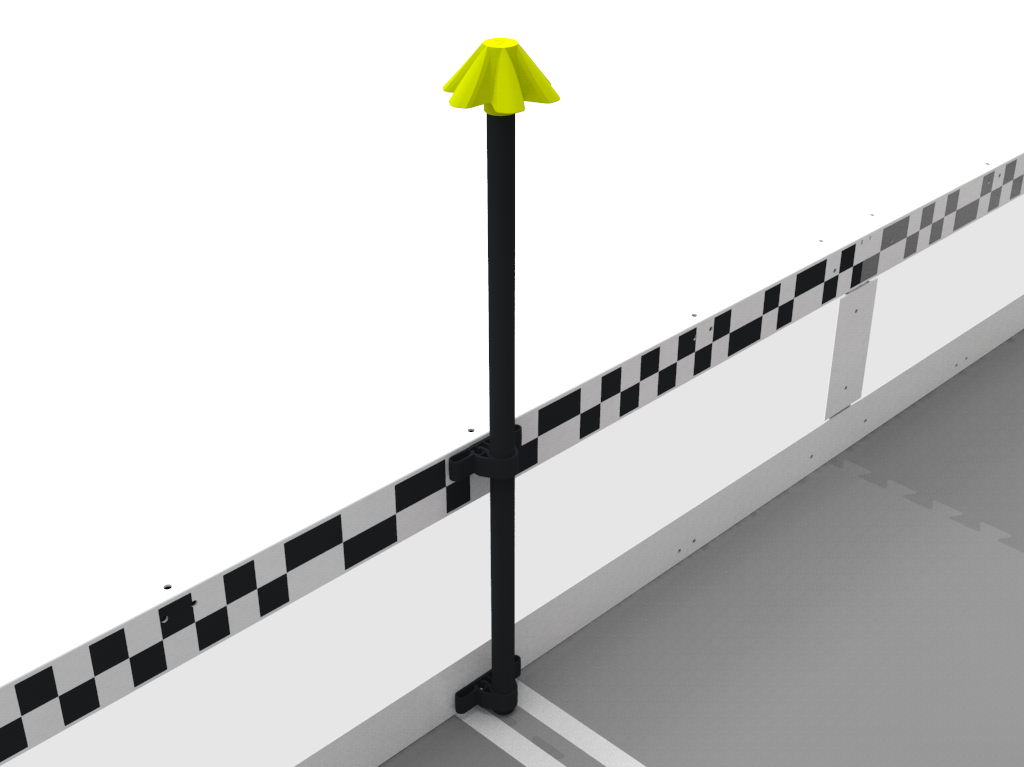
\includegraphics[width=0.5\linewidth]{images/Neutral Stake.png}
    \caption{Neutral Stake}
    \label{fig:neutral-stake}
\end{figure}
\section*{Solution Requirements}
\begin{itemize}
    \item This mechanism would need to use pneumatics, we don't have any motors to spare
    \item This mechanism needs to have at least 70\% accuracy 
    \item We need to stay within the 18 x 18 x 18 space restrictions 
\end{itemize}
\section*{Solution Goals}
\begin{itemize}
    \item We want to create something intuitive and easy for Chase to use
\end{itemize}
\brainstorm{Brainstorm \& Diagram: Arm V1.0 (September 1st, 2024)}
\info{Caleb Bachmeier}{Arm V1.0}{September 1st, 2024}
\chapterauthor{Caleb Bachmeier}
\section*{Possible Solutions}

\noindent
\textbf{Redirect}:

A redirect system would a Ring from our Intake and move it into a claw, this would then be raised and forced onto the Neutral Stake. Like in this prototype built by \textit{Drumroll Please Robotics} "\cite{Drumroll}" in Figure \ref{fig:drumroll} or would be very similar to 1010W's Arm "\cite{1010W}." As shown in Figure \ref{fig:1010W-arm}
\begin{figure}[H]
    \centering
    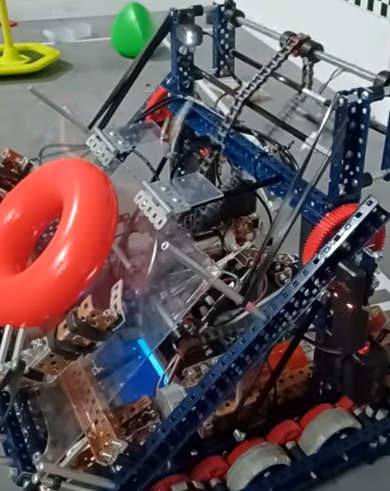
\includegraphics[width=0.5\linewidth]{images/Drumroll Redirect.png}
    \caption{3131V's Redirect}
    \label{fig:drumroll}
\end{figure}

\begin{figure} [H]
    \centering
    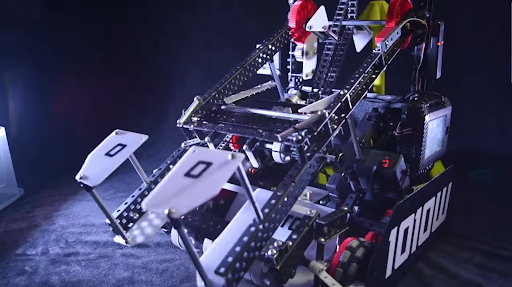
\includegraphics[width=0.5\linewidth]{images/1010W Arm.png}
    \caption{1010W Early Season Arm}
    \label{fig:1010W-arm}
\end{figure}


\noindent
\textbf{Pros}:
\begin{itemize}
    \item Chase wouldn't have to worry about picking the Rings off of the ground with a Claw
    \item We wouldn't need to use either pnuematics nor motors  
\end{itemize}
\textbf{Cons}:
\begin{itemize}
    \item It could be hard to code 
    \item Depending on the way we create it, it could be hard to drive
\end{itemize}

\noindent
\textbf{Outward Facing C-Channel}:

We could also do something similar to the Hero Bot for High Stakes "Axel" as shown in Figure \ref{fig:Axel} . This would use Tank Treads (SKU: 276-2214) \vex

\begin{figure}[H]
    \centering
    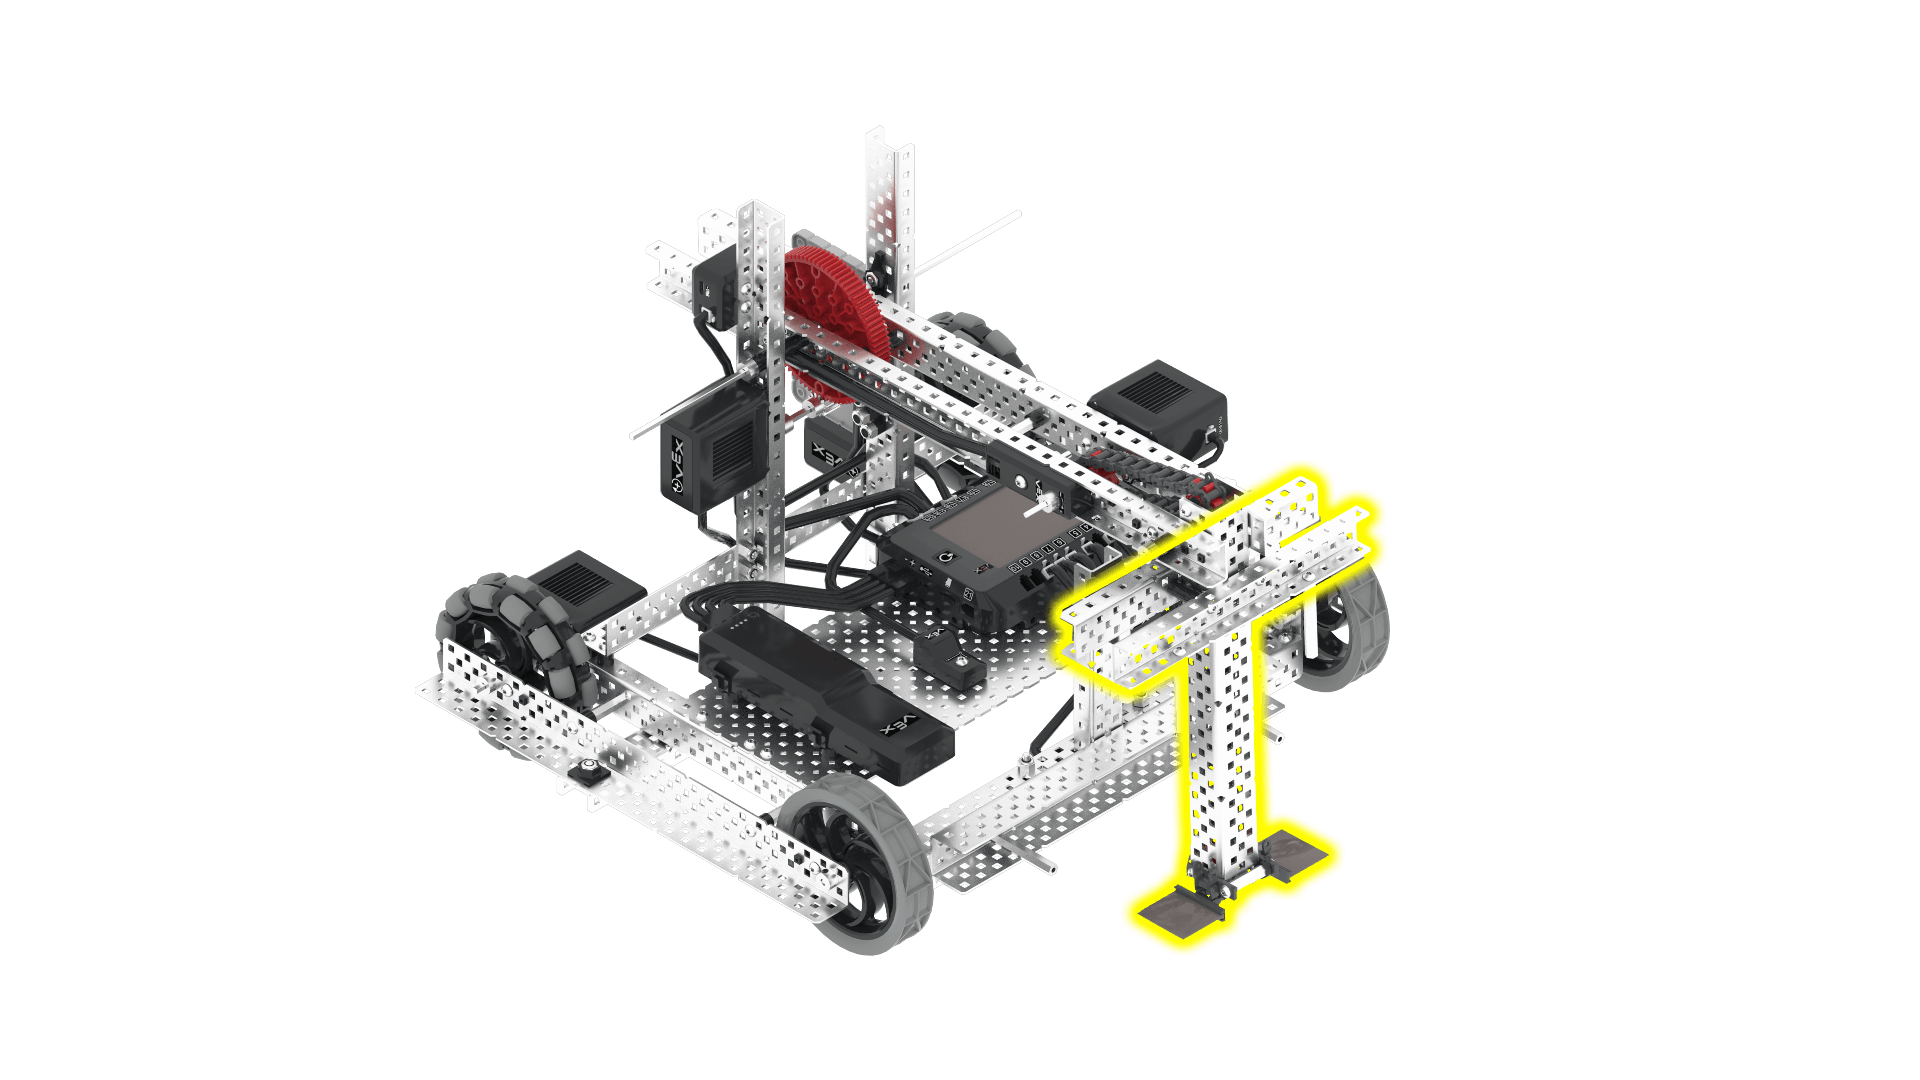
\includegraphics[width=0.7\linewidth]{images/Hero Bot Arm.png}
    \caption{"Axel's" Outward Facing C-Channel}
    \label{fig:Axel}
\end{figure}
\noindent
\textbf{Pros}:
\begin{itemize}
    \item This would be really easy to create
\end{itemize}
\textbf{Cons}:
\begin{itemize}
    \item It would probably go outside our 18 x 18 x 18 constrictions 
    \item We would have to figure out a way to mount it on top of our robot
    \item It might be hard to use pneumatics with this design
\end{itemize}

\solution{Choose a Solution: Arm V1.0 (September 1st, 2024)}
\info{Caleb Bachmeier}{Arm V1.0}{September 1st, 2024}
\chapterauthor{Caleb Bachmeier}
\section*{Choose a Solution}
\renewcommand{\arraystretch}{1.85} % Change this value as needed
\begin{table}[htb!]
\centering
\begin{tabular}{|>{\centering\arraybackslash}m{1.85cm}|>{\centering\arraybackslash}m{1.85cm}|>{\centering\arraybackslash}m{1.85cm}|>{\centering\arraybackslash}m{1.85cm}|>{\centering\arraybackslash}m{1.85cm}|>{\centering\arraybackslash}m{1.85cm}|>{\centering\arraybackslash}m{1.85cm}|}
\hline
\textbf{Scale 1 - 10} & \textbf{Complexity} & \textbf{Power} & \textbf{Reliability} & \textbf{Size} & \textbf{Speed} & \textbf{Total} \tabularnewline
\hline
Weight & x1 & x3 & x3 & x2 & x2 & \tabularnewline
\hline
Redirect & 3 & 10 & 7 & 8 & 8 & 86 \tabularnewline
\hline
Axel's Arm & 8 & 5 & 7 & 9 & 6 & 74 \tabularnewline
\hline
\end{tabular}
\caption{Drive Decision Matrix}
\label{tab:drive-matrix}
\end{table}
\renewcommand{\arraystretch}{1.85} % Reset to default
It seems that a redirect system would work best. Let's make a plan.
\build{Build \& Program: Arm V1.0 (September 1st, 2024)}
\info{Connor Albers}{Arm V1.0}{September 1st, 2024}
\chapterauthor{Connor Albers}
\section*{Building}
\section*{The Arm Mechanism}

The first component we needed to engineer was the arm. Our mechanism needed to use pneumatics as opposed to motors. This was necessary because we had already used all of our motors, with six on our drive and two on our intake. Our arm pivoted off the top high-strength axle of our intake because adding any additional axles would have required us to wrap our chain around them to prevent our hooks from catching.

\section*{The Arm Structure}

Our arm consisted of two C-channels, each with a 75mm piston attached. This is shown in Fusion 360 in \ref{fig:redirect-pnuematics}
\begin{figure}[H]
    \centering
    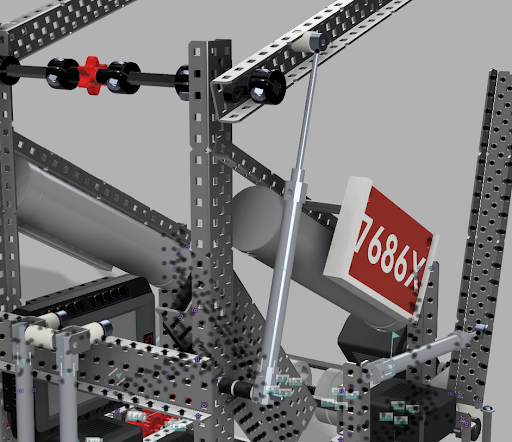
\includegraphics[width=0.5\linewidth]{images/CAD Redirect Pnuematics.png}
    \caption{Redirect Pnuematics}
    \label{fig:redirect-pnuematics}
\end{figure}
We positioned our pistons so they were mounted on the arm as far away from the pivot as possible to gain the most leverage. In doing this, we also ensured that our arm’s range of motion was not limited too much, allowing the arm to still reach high enough to score on the neutral stakes.

\section*{The Basket Construction}

After finishing the primary structure, it was time to construct the basket the rings would be redirected into. This consisted of two 15-hole-long C-channels that pivoted on the end of the main two C-channels. This is shown in Figure \ref{fig:armc-channels}
\begin{figure}[H]
    \centering
    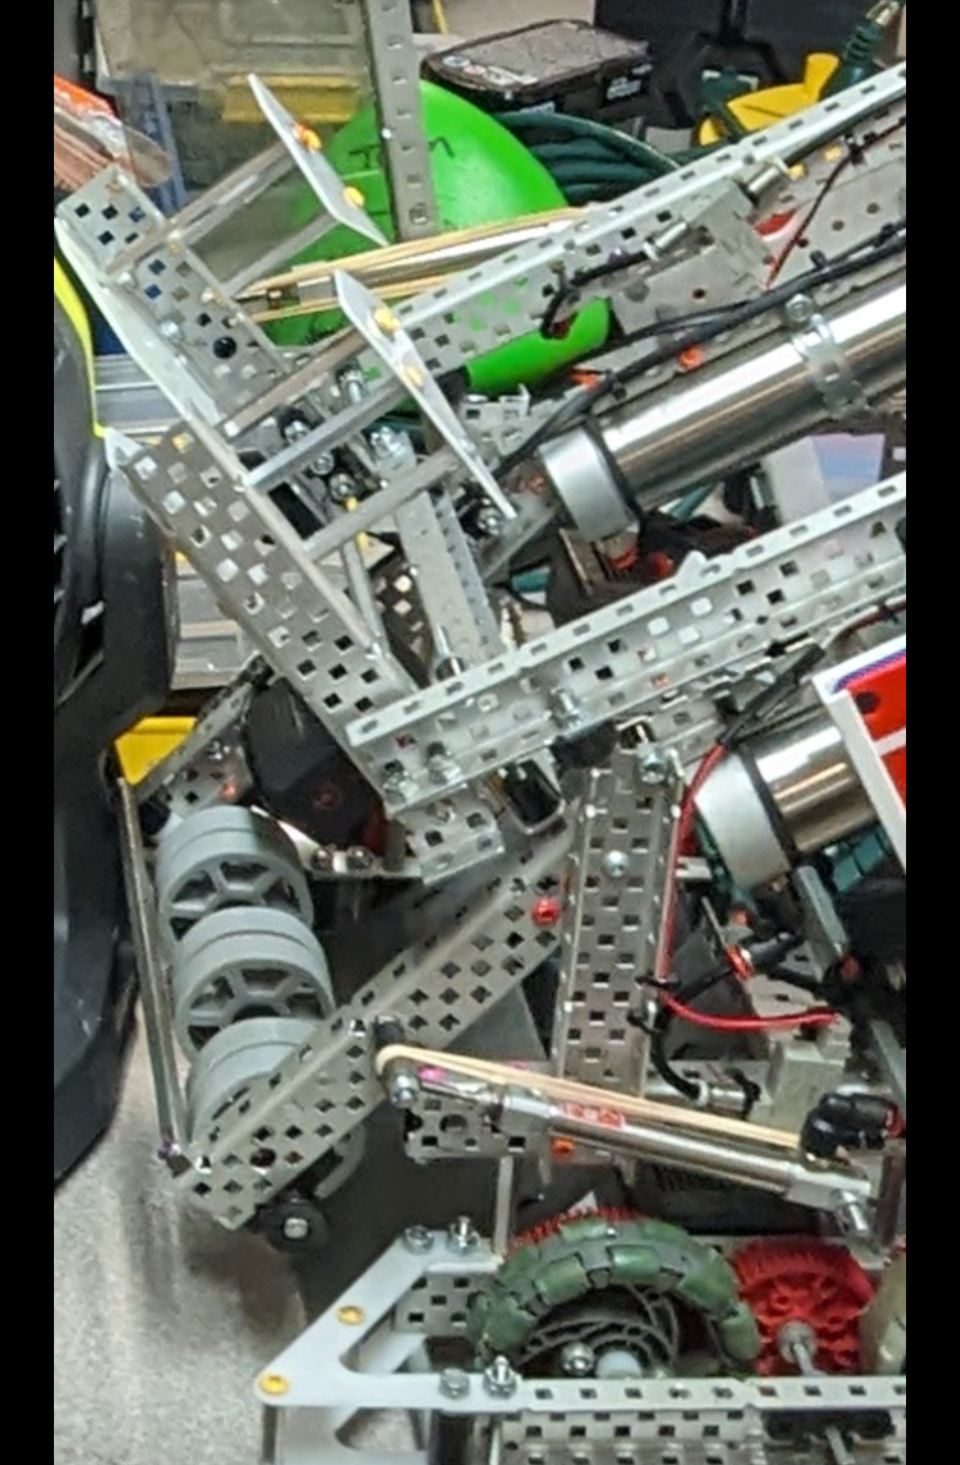
\includegraphics[width=0.5\linewidth]{images/Armc-channels.png}
    \caption{C-channels}
    \label{fig:armc-channels}
\end{figure}

After building that, we needed to connect the two sides of the arm. To reduce weight and because most of the interior of the arm needed to be clear, we decided to include only one cross brace, which crossed over both sides of the pivoting baskets. 

\section*{Connecting the Basket}

This cross brace not only connected both sides of the basket but, because the basket was rigidly attached to the main C-channels using screw joints, also connected the two main C-channels of the arm. For this cross brace, we decided to use a custom-cut and drilled high-strength axle because of its exceptional strength. After both sides were connected, the next step was to add a pneumatic system that would allow the basket to flip with the press of a button. This feature was mandatory for our design because, without it, we would be out of starting size.

\section*{Basket Support Pieces}

The final pieces of the basket were two custom-cut acetal pieces to support the rings in the basket. This is shown better in Figure \ref{fig:redirect-basket}
\begin{figure}[H]
    \centering
    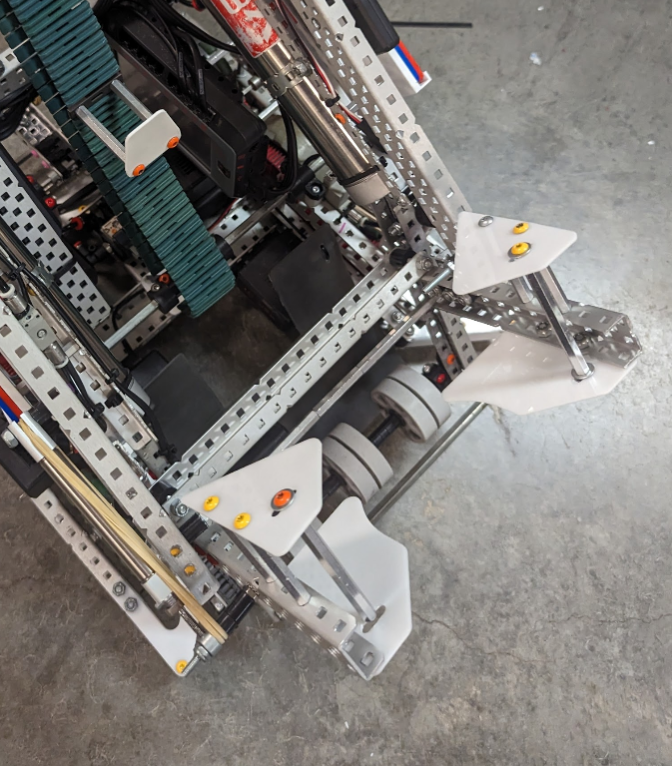
\includegraphics[width=0.5\linewidth]{images/Redirect-Basket.png}
    \caption{Basket for Rings}
    \label{fig:redirect-basket}
\end{figure}
These pieces provided maximum clearance for the stake to pass through the ring and allowed the ring to glide freely into the basket. The top pieces were offset using standoffs to give the basket a capacity of two rings. 

\section*{The Redirect Ramp}

The final piece of our redirect was the one-way ramp that allowed rings to slide into the basket. This is the point in construction where we encountered issues. The problem with this ramp was that the angle needed to be steep enough to make the rings slide down it. This proved problematic because we couldn't achieve this angle. A key factor contributing to this problem was the basket resting too high relative to our intake, which meant the angle of the ramp was too shallow to allow the rings to slide on their own.

\section*{Modifying the Ramp}

Unfortunately, because the stopper that determined the height at which our arm rested was our intake tower, the only solution was to limit the capacity of our redirect to one ring. Implementing this was simple—we just shortened the standoffs that offset the top acetal retaining pieces. After mocking up the ramp’s placement again, we realized this mechanism might not be the best solution for our current robot design because the ramp angle was still too shallow for the rings to slide.

\section*{Reconsidering the Mechanism}

At this point, we had seen concepts from other teams that appeared to be much faster than this solution and would work better given our current design. For now, we will disregard the Redirect mechanism and create another Engineering Design Process to create a Arm mechanism. This is in \blueref{chap:ArmV1.1}{Arm EDP V1.1}  \footnote{Added September 30, 2024}

